\chapter{\uppercase{Second Publishable Paper} \label{chapter:03}}

\section{Summary}
Abstract from second publishable paper.

\section{Intro}

Hey, remember in Chapter~\ref{chapter:02} when I said you'll have to repeat
yourself?  Well, \eqref{eq:chap2_example_eq} and \eqref{eq:chap3_example_eq}
should look the same, but have different \LaTeX\ labels an be referenced
correctly.

\begin{equation}
\label{eq:chap3_example_eq}
  \omega_{jk}\left(x\right) =
  \begin{cases}
  \hfil 0                                        & \hfil x \leq \xi_{j} \\
  \frac{x - \xi_{j}} {\xi_{j + k - 1} - \xi_{j}} & \xi_{j} < x < \xi_{j+ k - 1} \\
  \hfil 1                                        & \hfil \xi_{j + k - 1} \leq x
  \end{cases}.
\end{equation}

\section{Details}
\lipsum
 
\begin{figure}
\centering
  \begin{subfigure}[t]{0.48\linewidth}
  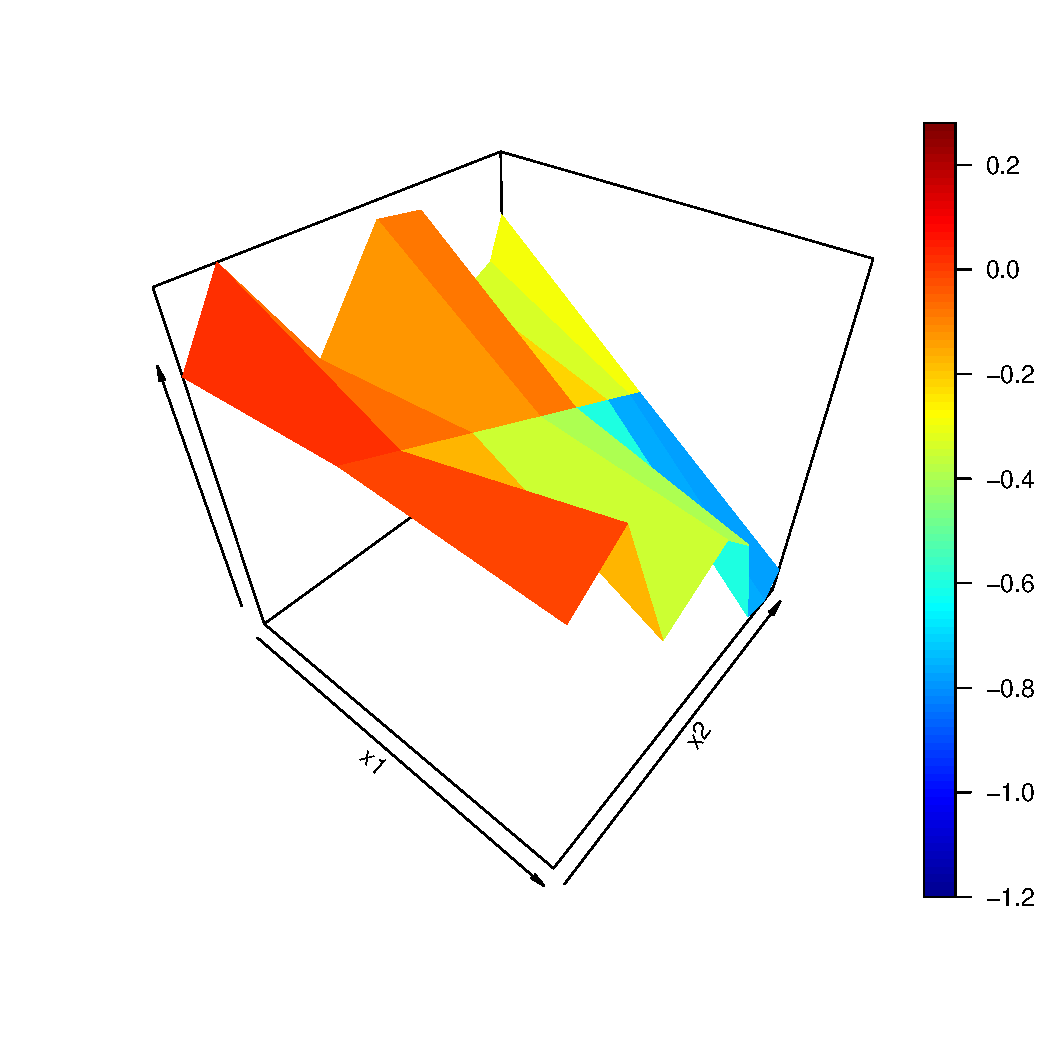
\includegraphics[width=\linewidth]{figures/c}
  \caption{\label{fig:graphic_c}}
  \end{subfigure}
  ~
  \begin{subfigure}[t]{0.48\linewidth}
  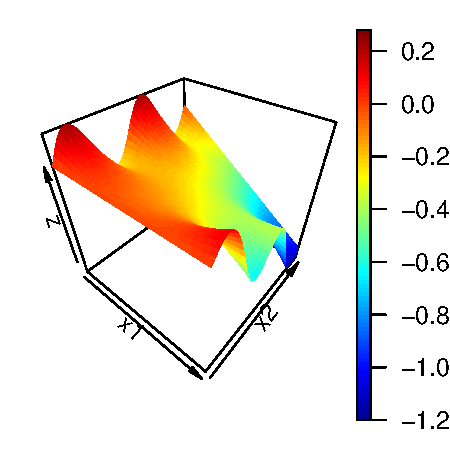
\includegraphics[width=\linewidth]{figures/d}
  \caption{\label{fig:graphic_d}}
  \end{subfigure}
  \caption[Another short caption for List of Figures]{Long Caption with lots of details
  \ldots \label{fig:chap3_graphic}}
\end{figure}

\section{Discussion}
\lipsum


